%\begin{figure}[h]
%\begin{minipage}[h]{0.3\linewidth}
%\center{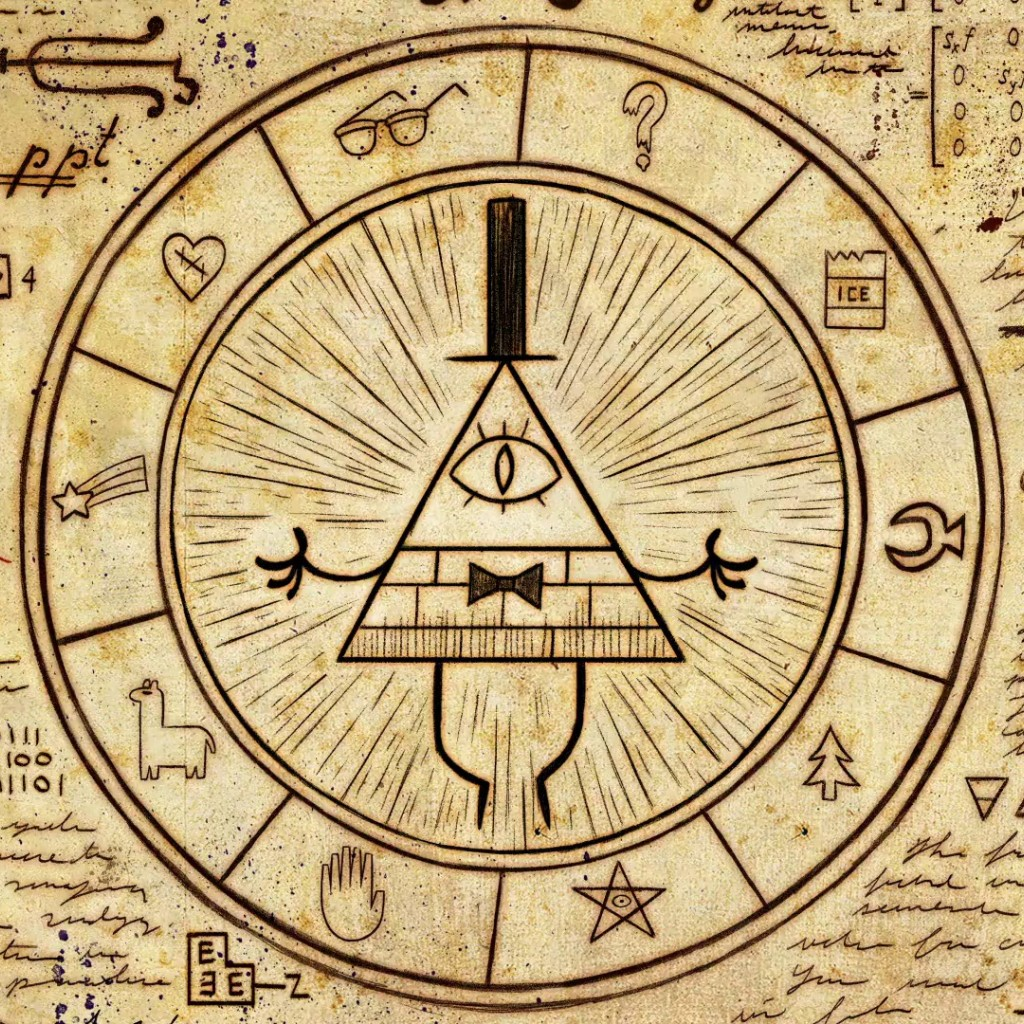
\includegraphics[width=\linewidth,natwidth=1024,natheight=1024]{Bill.jpg} \\}
%\end{minipage}
%\begin{minipage}[h]{0.3\linewidth}
%\center{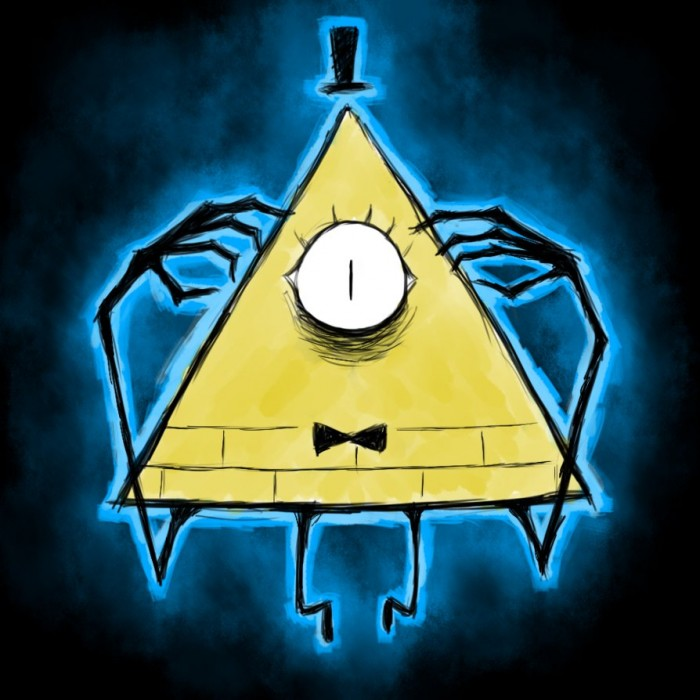
\includegraphics[width=\linewidth,natwidth=700,natheight=700]{Bill2.jpg} \\}
%\end{minipage}
%\begin{minipage}[h]{0.3\linewidth}
%\center{
\includegraphics[width=\linewidth,natwidth=512,natheight=512]{Bill3.jpg} \\}
%\end{minipage}
%\end{figure}

Билл Шифр решил захватить наш мир. Для этого ему нужны могущественные союзники, но он привык ни на кого не полагаться, кроме самого себя. Поэтому после недолгих раздумий Билл пришел к выводу, что самым лучшим решением будет он сам. Так как Шифр обладает огромной силой, создание армии своих собственных клонов не составит для него никакого труда. Но вот незадача, в нашем мире магия очень нестабильна, а значит появление больших летающих треугольников может происходить лишь в строго ограниченном наборе точек пространства. Билл Шифр знает координаты всех мест, в которых может зародится один из углов его творения, но хочет узнать, какие точки будут лучшими для создания его огромных версий. Помогите Биллу узнать координаты точек, в которых получится создать наибольшего по размеру Билла Шифра (наибольший по размеру~---~имеющий наибольший периметр). 

\InputFile
В первой строке подается число  $N$, ($1 \le N \le 100$)~---~количество точек для создания треугольников. Затем в каждой из $N$ строк идут координаты точек~---~ вещественные числа $X(-1000 \le X \le 1000)$ и $Y(-1000 \le Y \le 1000)$. Точность знаков соблюдать до $10^{-4}$.

\OutputFile
Выведите координаты наибольшего треугольника. Если их несколько, то выведите любые из них. 

\SAMPLES
